\documentclass[conference]{IEEEtran}
\IEEEoverridecommandlockouts
% The preceding line is only needed to identify funding in the first footnote. If that is unneeded, please comment it out.
\usepackage{cite}
\usepackage{amsmath,amssymb,amsfonts}
\usepackage{algorithmic}
\usepackage{graphicx}
\usepackage{textcomp}
\usepackage{siunitx}
\usepackage{xcolor}
\def\BibTeX{{\rm B\kern-.05em{\sc i\kern-.025em b}\kern-.08em
    T\kern-.1667em\lower.7ex\hbox{E}\kern-.125emX}}
\begin{document}

\title{MECH0010 Assignment Report 1
}

\author{\IEEEauthorblockN{Hasha Dar}
\IEEEauthorblockA{
hasha.dar.19@ucl.ac.uk}
\and
\IEEEauthorblockN{Christopher Tawk}
\IEEEauthorblockA{
christopher.tawk.19@ucl.ac.uk}
\and
\IEEEauthorblockN{Xichen Yang}
\IEEEauthorblockA{
xichen.yang.19@ucl.ac.uk}
}

\maketitle

\section{Question 1}
In the real world, the operation of DC motor is the transfer from electrical energy to the mechanical rotation of motor. Therefore, the electric circuit of motor operation is composed by the input voltage ($v$ (\si{\volt})), terminal resistance ($R$ (\si{\ohm})), Inductance ($L$ (\si{\henry})), and the electromotive force ($em$ (\si{\volt})). In this case the formulas for the time domain and frequency domain are ($i$ is the current of the circuit):
\begin{align}
    V &= Ri + L \frac{\textrm{d}i}{\textrm{d} t} + em\\
    V(s) &= RI(s) + LsI(s) + Em(s) \label{ll1}
\end{align}

For the mechanical rotation, the relationship among torque ($T$ (\si{\newton\metre})), moment of inertia ($Im$ (\si{\kg\metre\squared})), angular displacement ($\theta$) and the friction coefficient ($b$) in time domain and frequency domain are given:
\begin{align}
    T &= Im \frac{\textrm{d}^2 \theta}{\textrm{d} t^2} + b \frac{\textrm{d} \theta}{\textrm{d} t}\\
    T(s) &= Ims^2 \theta(s) + bs\theta(s)\label{ll2}
\end{align}

In this case, angular velocity is proportional to the electromotive force and current is proportional to the torque of the motor. ($K_e$ the electrical motor constant, $K_t$ is the mechanical motor constant):
\begin{align}
    em &= K_e \frac{\textrm{d} \theta}{\textrm{d} t}\\
    Em(s) &= K_e s \theta(s)\\ \label{ll3}
    T &= K_t i\\
    T(s) &= K_t I(s) \label{ll4}
\end{align}

To find the response between angular position ($\theta$) and input voltage ($v$) in time domain, the Laplace transfer function by combination of Eq.\ref{ll1}, \ref{ll2}, \ref{ll3}, \ref{ll4} is shown below:
\begin{align}
    \frac{\theta (s)}{v(s)} = \frac{K_t}{bR_s (\frac{K_e K_t}{bR}) + \tau_e \tau_m s^2 + \tau_m s + \tau_e s +1}
\end{align}

Note: $\tau_m$ is the mechanical time constant of motor ($\tau_m=\frac{Im}{b}$), $\tau_e$ is the electrical time constant ($\tau_e=\frac{L}{R}$).

Assumption: Because the electrical time constant ($\tau_e$) is much smaller compared to the mechanical time constant of the motor ($\tau_m$), term $\tau_e\tau_ms^2$ and $\tau_es$ are approximately equal to zero compared with other terms. Therefore, the equation will become:
\begin{align}
    \resizebox{.43 \textwidth}{!}
    {$
    \frac{\theta (s)}{v(s)} = \frac{K}{s(\tau s + 1)} \ \left( K = \frac{K_t}{bR + K_t K_e}, \ \tau = \frac{\tau_m Rb}{K K_t + Rb} \right)
    $}
\end{align}

Due to the angular velocity ($\omega$) is the first derivative of angular position related to time ($\omega\left(s\right)=s\cdot\theta\left(s\right)$). In this case, the transfer function of angular velocity and input voltage is:
\begin{align}
    \frac{\omega(s)}{v(s)} = \frac{k}{\tau s + 1}
\end{align}

According to the specification data of Motor C42-L50 winding code 10 

\begin{table}[htbp]
    \caption{Specification Data}
    \begin{center}
    \begin{tabular}{|c|c|}
    \hline
    \textbf{Specification} & \textbf{Value}\\
    \hline
    \hline
    Torque sensitivity ($K_t$) & \SI{0.1412}{\newton\metre\per\ampere}\\
    \hline
    Back e.m.f. ($K_e$) & \SI{0.1413}{\volt\per\radian\per\second}\\
    \hline
    Rotor inertia ($Im$) & \SI{6.3354e-4}{\kg\per\meter\squared}\\
    \hline
    Mec. time constant ($\tau_m$) & \SI{0.0223}{\second}\\
    \hline
    Terminal resistance ($R$) & \SI{0.7}{\ohm}\\
    \hline
    Friction coefficient $\left(\frac{I_m}{\tau_m}\right)$ & \SI{0.0285}{}\\
    \hline
    \end{tabular}
    \label{sdtable}
    \end{center}
\end{table}

Therefore, the constant $K$ and overall time constant $\tau$ can be calculated as:
\begin{align}
    K = \frac{K_t}{bR + K_t K_e} &= 3.54\\ 
    \tau = \frac{\tau_m Rb}{K K_t + Rb} &= 0.0112
\end{align}

In this case, the transfer function of angular velocity and angular displacement of motor with voltage input is:
\begin{align}
    \frac{\omega (s)}{v(s)} = \frac{K}{(\tau s +1)} &= \frac{3.54}{0.0112s + 1}\\
    \frac{\theta (s)}{v(s)} = \frac{K}{s(\tau s + 1)} &= \frac{3.54}{0.0112s^2 + s}
\end{align}

where 3.54 is the gain of the system.

\begin{figure}[htbp]
    \centering
    \begin{minipage}[b]{0.24\textwidth}
      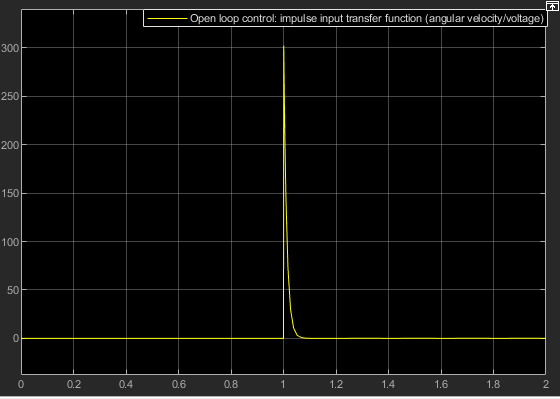
\includegraphics[width=\textwidth]{./Graph/G1.png}
      \caption{Model of open loop transfer function of angular velocity with impulse input.}
    \end{minipage}
    \hfill
    \begin{minipage}[b]{0.24\textwidth}
      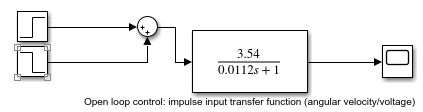
\includegraphics[width=\textwidth]{./Graph/Graph1.png}
      \caption{Model of open loop transfer function of angular velocity with step input.}
    \end{minipage}
\end{figure}





















\begin{figure}[htbp]
    \centerline{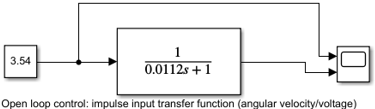
\includegraphics[width = 0.4\textwidth]{../img/q1-2.png}}
    \caption{Model of open loop transfer function of angular velocity.}
\end{figure}

\begin{figure}[htbp]
    \centerline{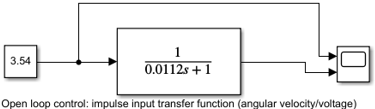
\includegraphics[width = 0.4\textwidth]{../img/q1-2.png}}
    \caption{Model of open loop transfer function of angular displacement.}
\end{figure}

\begin{figure}[htbp]
    \centering
    \begin{minipage}[b]{0.24\textwidth}
      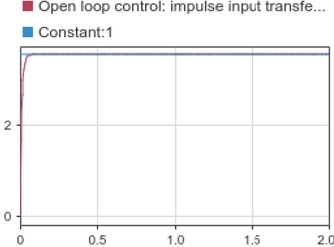
\includegraphics[width=\textwidth]{../img/q1-1.png}
      \caption{Model of open loop transfer function of angular velocity with impulse input.}
    \end{minipage}
    \hfill
    \begin{minipage}[b]{0.24\textwidth}
      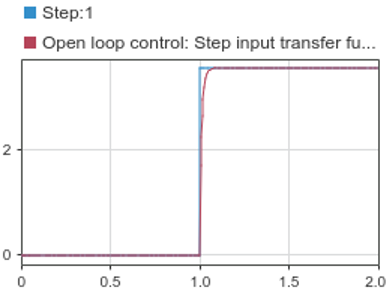
\includegraphics[width=\textwidth]{../img/q1-3.png}
      \caption{Model of open loop transfer function of angular velocity with step input.}
    \end{minipage}
\end{figure}

\begin{figure}[htbp]
    \centering
    \begin{minipage}[b]{0.24\textwidth}
      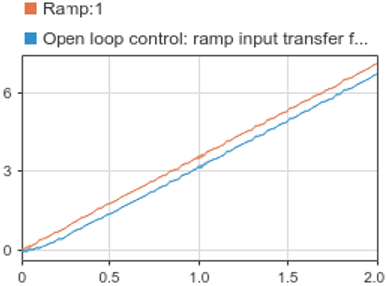
\includegraphics[width=\textwidth]{../img/q1-5.png}
      \caption{Model of open loop transfer function of angular velocity with ramp input.}
    \end{minipage}
    \hfill
    \begin{minipage}[b]{0.24\textwidth}
      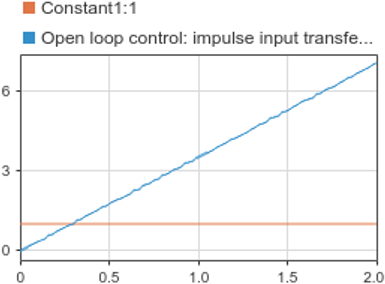
\includegraphics[width=\textwidth]{../img/q1-7.png}
      \caption{Model of open loop transfer function of angular displacement with impulse input.}
      \label{oltad1}
    \end{minipage}
\end{figure}

\begin{figure}[htbp]
    \centering
    \begin{minipage}[b]{0.24\textwidth}
      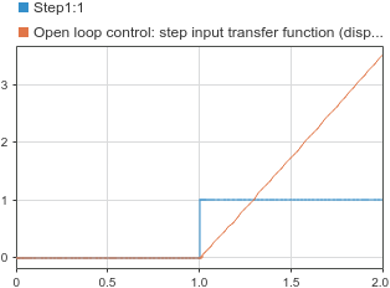
\includegraphics[width=\textwidth]{../img/q1-9.png}
      \caption{Model of open loop transfer function of angular displacement with step input.}
      \label{oltad2}
    \end{minipage}
    \hfill
    \begin{minipage}[b]{0.24\textwidth}
      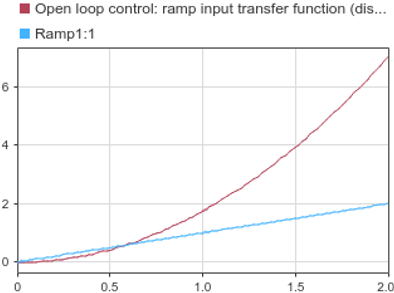
\includegraphics[width=\textwidth]{../img/q1-10.png}
      \caption{Model of open loop transfer function of angular displacement with ramp input.}
      \label{oltad3}
    \end{minipage}
\end{figure}

According to the results show in Graphs.\ref{oltad1}, .\ref{oltad2}, .\ref{oltad3}, the response of output angular displacement will intersect with input and then overshoot to infinity (undesirable behaviour), which means these open loops cannot meet the requirement to control the angular displacement of the motor. Under this circumstance, the unit feedback closed loop with a gain of $H$ is required to overcome this undesirable behaviour of open loop control system for angular velocity. The formula for the feedback loop is:
\begin{align}
    G(s) &= \frac{\theta (s)}{v(s)} = \frac{3.54}{0.0112s^2 + s}\\
    H(s) &= H\\
    G'(s) &= \frac{G(s)}{1 + G(s) \cdot H(s)}
\end{align}

Therefore, the new transfer function is:
\begin{align}
    G'(s) &= \gamma \frac{\omega_n^2}{s^2 + 2\zeta \omega_n s + \omega_n^2}
\end{align}
\begin{align}
    \resizebox{.43 \textwidth}{!}
    {$
    G'(s) = \frac{316.07H}{H\left( s^2 + 2 \cdot 44.64 \cdot \sqrt{\frac{1}{316.07H}} \cdot \sqrt{316.07 H} s + 316.07 H\right)}
    $}
\end{align}

Note: $\gamma = \frac{1}{H}$, $\zeta = 44.64 \sqrt{\frac{1}{316.07H}}$ and $\omega_n = \sqrt{316.07H}$

In this case, we can use $\zeta$ to determine the response wanted as overdamped, critically damped, underdamped or undamped to control the loop without undesired behaviour and according to the results and analysis of transfer function of angular velocity, step input is suitable to make the response reach the desired input compared to ramp input and impulse input. Therefore, the step input is the input for the new transfer function to overcome the undesirable behaviour. The results of the simulation for Simulink are shown in Fig.\ref{damp1}, \ref{damp2}, \ref{damp3}. 

\begin{figure}[htbp]
    \centerline{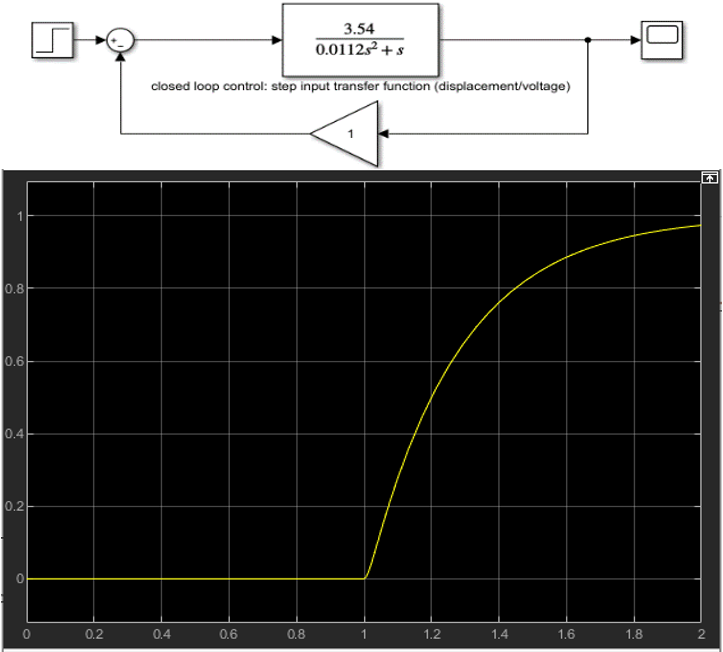
\includegraphics[width = 0.4\textwidth]{../img/q1-11.png}}
    \caption{Overdamped. $\zeta > 1$, $0 < H < 6.304 \therefore H = 1$}
    \label{damp1}
\end{figure}

\begin{figure}[htbp]
    \centerline{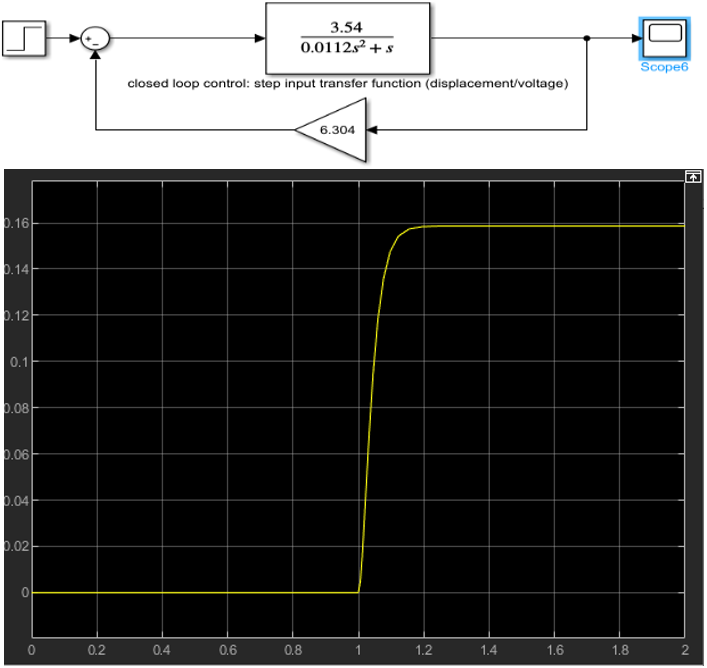
\includegraphics[width = 0.4\textwidth]{../img/q1-12.png}}
    \caption{Critically damped. $\zeta = 1$, $H = 6.304$}
    \label{damp2}
\end{figure}

\begin{figure}[htbp]
    \centerline{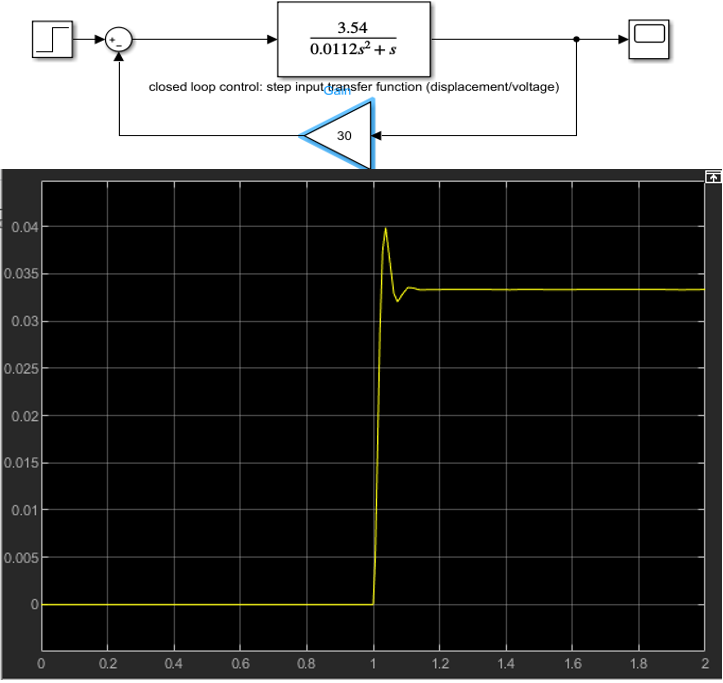
\includegraphics[width = 0.4\textwidth]{../img/q1-13.png}}
    \caption{Underdamped. $0 < \zeta < 1$, $H > 6.304$. In this case, $H = 30$}
    \label{damp3}
\end{figure}

There is no undamped condition in this case as $\omega_n$ also depends on $H$.

\section{Question 2}
\subsection{4}
Considering a FDM (fused deposition modelling) PLA (polyactic acid) 3D printer, typical printing speeds \cite{b1} for a medium end model are \SI{100}{\milli\meter\per\second}. The accuracy for a good printer would be around $\pm$\SI{0.2}{\milli\meter}. The sampling rate of an Arduino's analogue input port is roughly \SI{9600}{\hertz}, as tested here. This would allow us to have a strip with a blocked-transparent pattern in \SI{1}{\milli\meter} blocks (i.e. \SI{0.5}{\milli\meter} of blocked out and then \SI{0.5}{\milli\meter} of transparent). Assuming our sample rate is stable at \SI{9600}{\hertz}, if the head travels at \SI{100}{\milli\meter\per\second}, we will traverse 96 patterned blocks. This relates to 96 samples per block traversed. This should provide adequate information to measure the intensity of light from the LED. When the printer head moves along the encoder, the intensity of the light reaching the LDR will form a sinusoidal intensity signal. We can utilise a comparator to remove noise from our signal by inverting one of the outputs and running both signals to the inputs of an op-amp. This will be beneficial in reducing error signals, a necessary requirement for a high-accuracy system. 

We can measure which direction the head is moving in and the position of the head by using a quadrature sine/cosine signal. This is where we take the voltage signal from our LDR (a sinusoid) and compare it with a signal with a $\frac{\pi}{2}$ phase shift. Plotting these on an xy oscilloscope will produce a plot called a Lissajous figure. Under perfect conditions, our Lissajous figure will be a circle centred on the origin. The radius of the Lissajous is based on the amplitude and the direction in which the point is traced relates to whether our linear encoder is being read in the positive or negative direction. However, we may see that our Lissajous is not a perfect circle and this can be amended with trimming the signal and calibrations. The Lissajous figure tells us the position of the printer head, but we will need an absolute reference in order for our printer head to know where it is. For example, setting the zero point at the top right corner, we can count the number of times our Lissajous traverses $2\pi$ times in the oscilloscope, when the head moves. We can use the axis' crossed as a reference as to whether the number should be increased or decreased. As we also know the size of our strip pattern, we can derive the position of the head.

\begin{figure}[htbp]
    \centerline{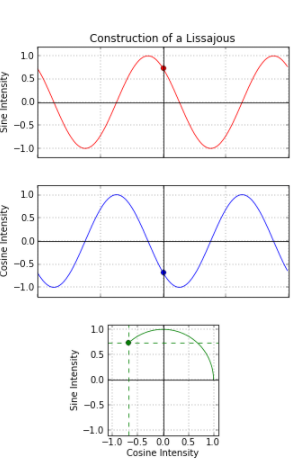
\includegraphics[width = 0.45\textwidth]{../img/Lissajous1.png}}
    \caption{Lissajous plot}
\end{figure}


\begin{thebibliography}{00}
\bibitem{b1} 3D printing, how to obtain the best possible speeds, Chris Joel, https://www.3dprintersonlinestore.com/how-to-obtain-best-3d-printing-speed Accessed at 28-11-20 16:14:32
\end{thebibliography}

\end{document}